\chapter{Metodologia e Sviluppo}
\label{ch:metodologiasviluppo}

In questo capitolo verrà presentata la metodologia e lo sviluppo delle soluzioni
proposte nel capitolo \ref{sec:soluzione} per l'ottimizzazione della libreria
\textit{CoopeRIS}. Verranno descritte le fasi di analisi, progettazione ed implementazione,
con particolare attenzione alle scelte effettuate e alle motivazioni che hanno
portato alla realizzazione delle stesse. Infine, sarà presente una discussione
sui vantaggi, svantaggi e limiti di ciascuna soluzione, oltre che alle sfide
affrontate durante lo sviluppo.

\section{Stato dell'arte della libreria \textit{CoopeRIS}}
\label{sec:libreria}

La libreria \textit{CoopeRIS} non è particolarmente complessa e rispecchia i
principi della programmazione ad oggetti. Tuttavia, presenta alcune criticità
nei metodi che implementa che ne limitano l'efficienza e la scalabilità, in particolare
nelle procedure di calcolo del \textit{guadagno} del segnale riflesso dalla RIS.
Questo sottocapitolo si propone di fornire una panoramica generale della libreria
in oggetto e delle sue funzionalità principali, oltre che la ricerca delle
possibili aree di ottimizzazione della stessa.

\subsection{Architettura e funzionamento}
\label{sec:architettura}

Il suo funzionamento è basato su un'architettura a classi in cui ogni istanza rappresenta
una RIS, i suoi metodi implementano le operazioni necessarie al fine di
calcolare le grandezze fisiche e geometriche utili alla simulazione, ed infine sfrutta
la libreria GSL\cite{gnugsl} per la manipolazione di vettori e matrici, reali e complesse.
Le due procedure principali sono le seguenti:

\begin{itemize}
  \item \texttt{computePhases}: calcola le fasi dei singoli elementi dati gli angoli
    di incidenza e riflessione;

  \item \texttt{gain}: calcola il guadagno isotropico del segnale riflesso dalla
    RIS dati gli angoli di trasmettitore e del ricevitore, diretta derivazione
    dell'equazione \ref{eq:gain}.
\end{itemize}

In una esecuzione tipica, la prima fase prevede di calcolare le fasi dati gli
angoli di incidenza e riflessione tramite la funzione \texttt{computePhases} salvandoli
sulla matrice denominata $coding$, ovvero lo stato degli elementi della RIS, per
poi calcolare il guadagno del segnale riflesso tramite il metodo \texttt{gain}.

\subsection{Identificazione dei colli di bottiglia e aree di ottimizzazione}
\label{sec:ottimizzazione}

Il metodo \texttt{computePhases} non è particolarmente soggetto a criticità, la sua
complessità computazionale è lineare rispetto al numero di elementi della RIS.
Inoltre, dopo una prima profilazione, la procedura risulta già essere
sufficientemente veloce e ottimizzata. Il metodo \texttt{gain}, osservabile nel dettaglio
nel listato \ref{lst:gain}, è invece più complesso e richiede un numero molto
maggiore di operazioni. La procedura di calcolo del guadagno è infatti basata su
un doppio ciclo $for$ annidato, che scorre tutti gli elementi della RIS e
calcola il contributo di ciascuno di essi al guadagno totale, per ogni possibile
elemento sferico, come in equazione \ref{eq:gain} e \ref{eq:power}. Questo comporta
che il metodo \texttt{gain} scali computazionalmente in maniera quadratica
rispetto al numero di elementi della RIS e alla scelta di discretizzazione dei
possibili angoli $\phi$ e $\theta$ (aumentando di conseguenza il numero di elementi
sferici).

\vspace{1em}
\lstinputlisting[caption=Metodo \texttt{gain} della libreria \textit{CoopeRIS}, language=C++,
label=lst:gain]{listings/original-gain.cpp}
\vspace{1em}

Dopo una prima analisi statica del codice, si possono identificare quali parti
di esso corrispondano alle operazione matematiche descritte nelle equazioni
\ref{eq:power} e \ref{eq:gain}:

\begin{itemize}
  \item Le righe 18-19 sono i due cicli $for$ annidati che scorrono tutti gli elementi
    della RIS, indicati dalle sommatorie in equazione \ref{eq:power};

  \item Le matrici $n\_k\_du\_sin\_cos$ e $m\_k\_du\_sin\_sin$ in righe 24-25 corrispondono
    rispettivamente ai termini $\Phi_{m,n}$ e $\Theta_{m,n}$, in questo caso
    precedentemente calcolati, per ogni possibile angolo discreto $\phi$ e $\theta$
    di trasmettitore, ricevitore, incidenza e riflessione, come equazione
    \ref{eq:power};

  \item Alle righe 35-36 è presente la moltiplicazione per $-j$ dei precedenti termini
    e l'applicazione della funzione esponenziale, come in equazione
    \ref{eq:power};

  \item A riga 38 si trova è la somma di $\textbf{P}_{\phi_{rx},\theta_{rx}}$ per
    elemento della RIS nella matrice \texttt{phase}, utile per il calcolo del guadagno
    totale $\texttt{p\_tot}$ utilizzato in equazione \ref{eq:gain};

  \item Le righe 59-61 corrispondono al calcolo del guadagno del segnale $\texttt
    {p\_tot}$ espresso da $\textbf{G}$ in equazione \ref{eq:gain}
\end{itemize}

Si può notare inoltre un layer di cache nelle righe 10-12 e 70, implementato in
quanto permette di evitare il ricalcolo di valori già calcolati in precedenza.

Considerando della Legge di Amdahl discussa nel capitolo \ref{sec:amdahl}, i due
cicli $for$ rappresentano la porzione del codice ottimale per le ottimizzazioni in
oggetto in quanto sarà quella che meglio beneficerà della parallelizzazione.
Inoltre, questa specifica sezione è ulteriormente vantaggiosa poiché tutte le iterazioni
sono indipendenti, tranne che per la somma finale nella matrice \texttt{phase},
e per questo è stato il punto di partenza per la progettazione delle soluzioni
proposte.

\section{Implementazione delle soluzioni proposte}
\label{sec:implementazione}

Le soluzioni proposte per l'ottimizzazione del metodo \texttt{gain} sono basate
su due approcci differenti: la parallelizzazione tramite \textit{multi-threading}
e la parallelizzazione su GPU. Entrambe presentano piccole differenze, ma
condividono lo stesso obiettivo: ridurre il tempo di esecuzione nel calcolo della
matrice \texttt{phase} nei $for$ annidati a righe 18-19 del codice
\ref{lst:gain} per calcolare la matrice \texttt{phase}. Identificata la sezione
del codice da ottimizzare, si è passati alla fase di progettazione. Per poter
rendere il codice più modulare, e permettere agli utenti di poter scegliere l'implementazione
più adatta al proprio hardware, ogni diversa implementazione (multi-threading,
CUDA e OpenCL) è stata delimitata da guardie pre-processore. Durante la
configurazione del progetto tramite un apposito script \texttt{configure},
tipico del sistema di compilazione di \textit{OMNeT++}, è possibile scegliere
quale implementazione utilizzare mediante le opzioni \texttt{--with-cuda} e \texttt{--with-opencl}.
Il paradigma della parallelizzazione tramite multi-threading è selezionato se non
diversamente specificato.

\subsection{Parallelizzazione tramite multi-threading}
\label{subsec:multithreading}

Per la parallelizzazione tramite multi-threading è stato scelto di utilizzare la
libreria \textit{libpthread} che implementa il supporto per i thread POSIX al fine
di poter sfruttare più core della CPU simultaneamente. Questa decisione è stata
presa per questioni di massima compatibilità in quanto essa è disponibile su
tutti i sistemi operativi UNIX-like.

Il primo passo è stato quello di definire come dividere il lavoro tra i thread. A
questo scopo, si è scelto di dividere equamente il numero di elementi della RIS
per ogni thread. Per facilitare la gestione dei parametri da passare ad ogni thread,
la matrice di elementi RIS \texttt{coding} è linearizzata, così da poter passare
ad ogni thread un indice \texttt{start} e \texttt{end} per la sezione di
elementi su cui esso dovrà lavorare. Poi, nella procedura ogni thread estrarrà i
due indici dato l'indice $\texttt{start}\le i < \texttt{end}$ tramite le formule
$m = \frac{i}{N}$ ed $n = i \bmod N$, dove $N$ è il numero di colonne della matrice
\texttt{coding}. In seguito si è definita una struttura dati che contenesse i parametri
da passare ad ogni istanza dei thread, visionabile nel listato
\ref{lst:thread-params}.

\vspace{1em}
\lstinputlisting[caption=Struttura dati per i parametri dei thread, language=C++,
label=lst:thread-params]{listings/thread-params-struct.cpp}
\vspace{1em}

In questa struttura, sono presenti i seguenti campi:

\begin{itemize}
  \item \texttt{ris}: un puntatore alla RIS su cui effettuare i calcoli (necessario
    poiché la routine di ogni thread deve necessariamente essere un metodo
    statico);

  \item \texttt{thetaTX\_rad}, \texttt{phiTX\_rad}, \texttt{thetaRX\_rad} e
    \texttt{phiRX\_rad}: azimuth ed elevazione di trasmettitore e ricevitore;

  \item \texttt{start} e \texttt{end}: indici di partenza e fine per la porzione
    di elementi della RIS da calcolare;

  \item \texttt{tmp\_phase}: puntatore alla matrice parziale su cui ogni thread scrive
    i propri risultati.
\end{itemize}

Dopo aver definito la struttura dati, si a definire la routine che ogni thread
dovrà eseguire, come mostrato nel listato \ref{lst:thread-routine}.

\vspace{1em}
\lstinputlisting[caption=Procedura eseguita da ogni thread per il calcolo di
\texttt{phase}, language=C++, label=lst:thread-routine]{listings/thread-routine.cpp}
\vspace{1em}

Questa procedura è in pratica una copia delle operazioni effettuate nei cicli
$fo r$ in \ref{lst:gain}, con la differenza che ogni thread lavorerà su una porzione
di elementi della RIS e salverà i risultati parziali nella matrice \texttt{tmp\_phase}.
Infine, nel listato \ref{lst:thread-creation}, si può osservare come vengono creati
i thread, come vengono passati i parametri e come vengono attesi alla fine dell'esecuzione.

\vspace{1em}
\lstinputlisting[caption=Funzione del calcolo di \texttt{phase}, language=C++, label=lst:thread-creation]{listings/gain-compute-phase.cpp}

\begin{figure}
  \centering
  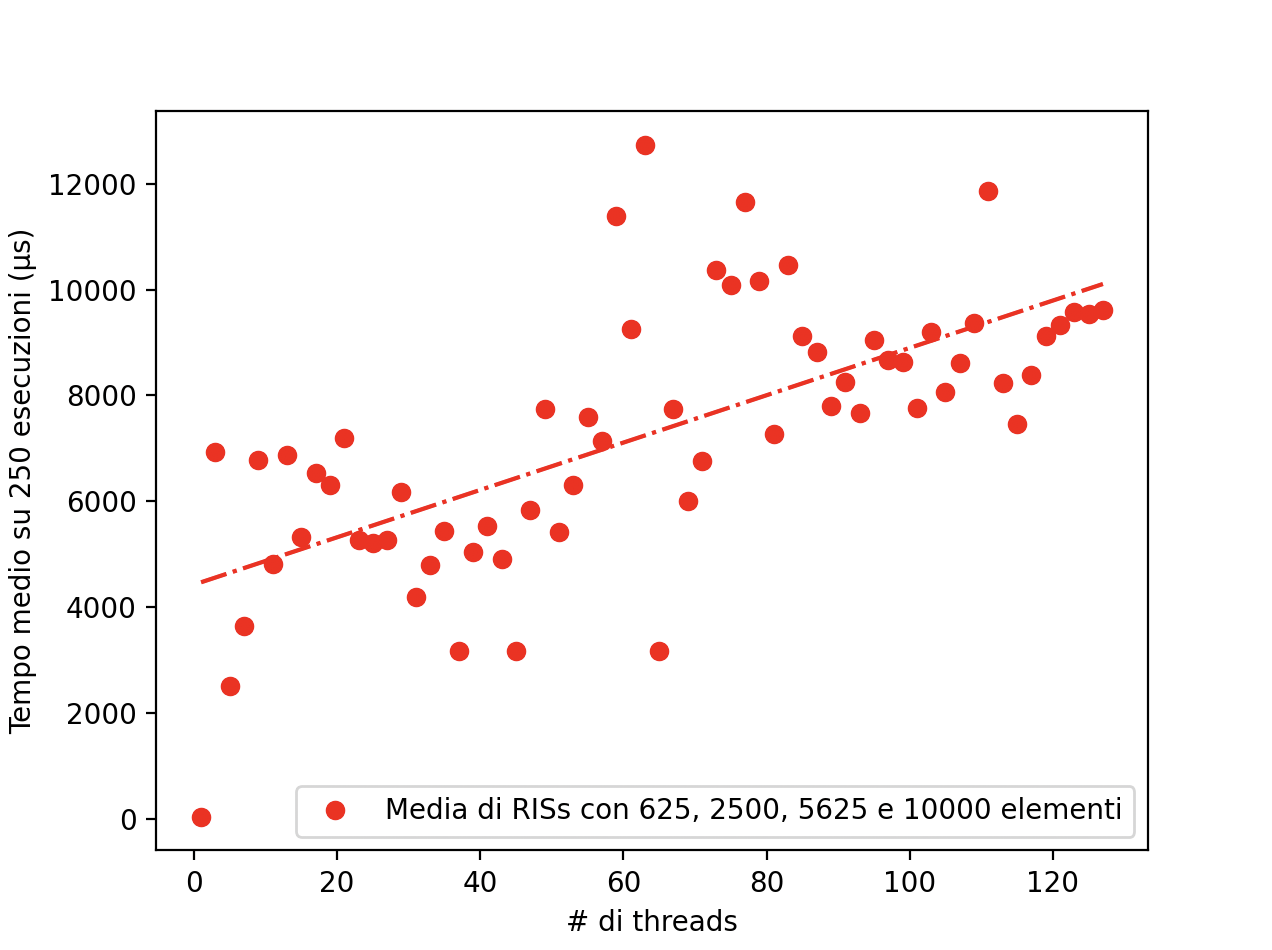
\includegraphics[width=.6\textwidth]{images/results/gain-serial-time.png}
  \caption{Delta del tempo di esecuzione tra la fine dell'ultimo thread e la
  fine della procedura \texttt{gain\_compute\_phase}}
  \label{fig:serial-time}
\end{figure}

Si vuole portare l'attenzione sulle righe 37-41: in questo $for$ si effettua l'attesa,
tramite la funzione \texttt{join}, e la somma dei risultati parziali di ogni
thread nella matrice \texttt{phase}. Anche se la procedura \texttt{gsl\_matrix\_complex\_add}
potrebbe sembrare un rallentamento, in realtà, tramite il \textit{pipelining}
delle operazioni di creazione dei thread, questo costo è ammortizzato e non influisce
significativamente sul tempo di esecuzione. In figura
\ref{fig:gain-compute-phase-pipeline} è possibile osservare una rappresentazione
grafica di questo processo: l'obiettivo è quello di assicurarsi che la procedura
tra $t_{4}$ e $t_{5}$ sia la più breve possibile, in modo da non rallentare l'intero
processo. In figura \ref{fig:serial-time} è possibile osservare le misurazioni di
$t_{5}- t_{4}$, che risulta essere con un trend crescente, ma comunque contenuto.

\begin{figure}
  \centering
  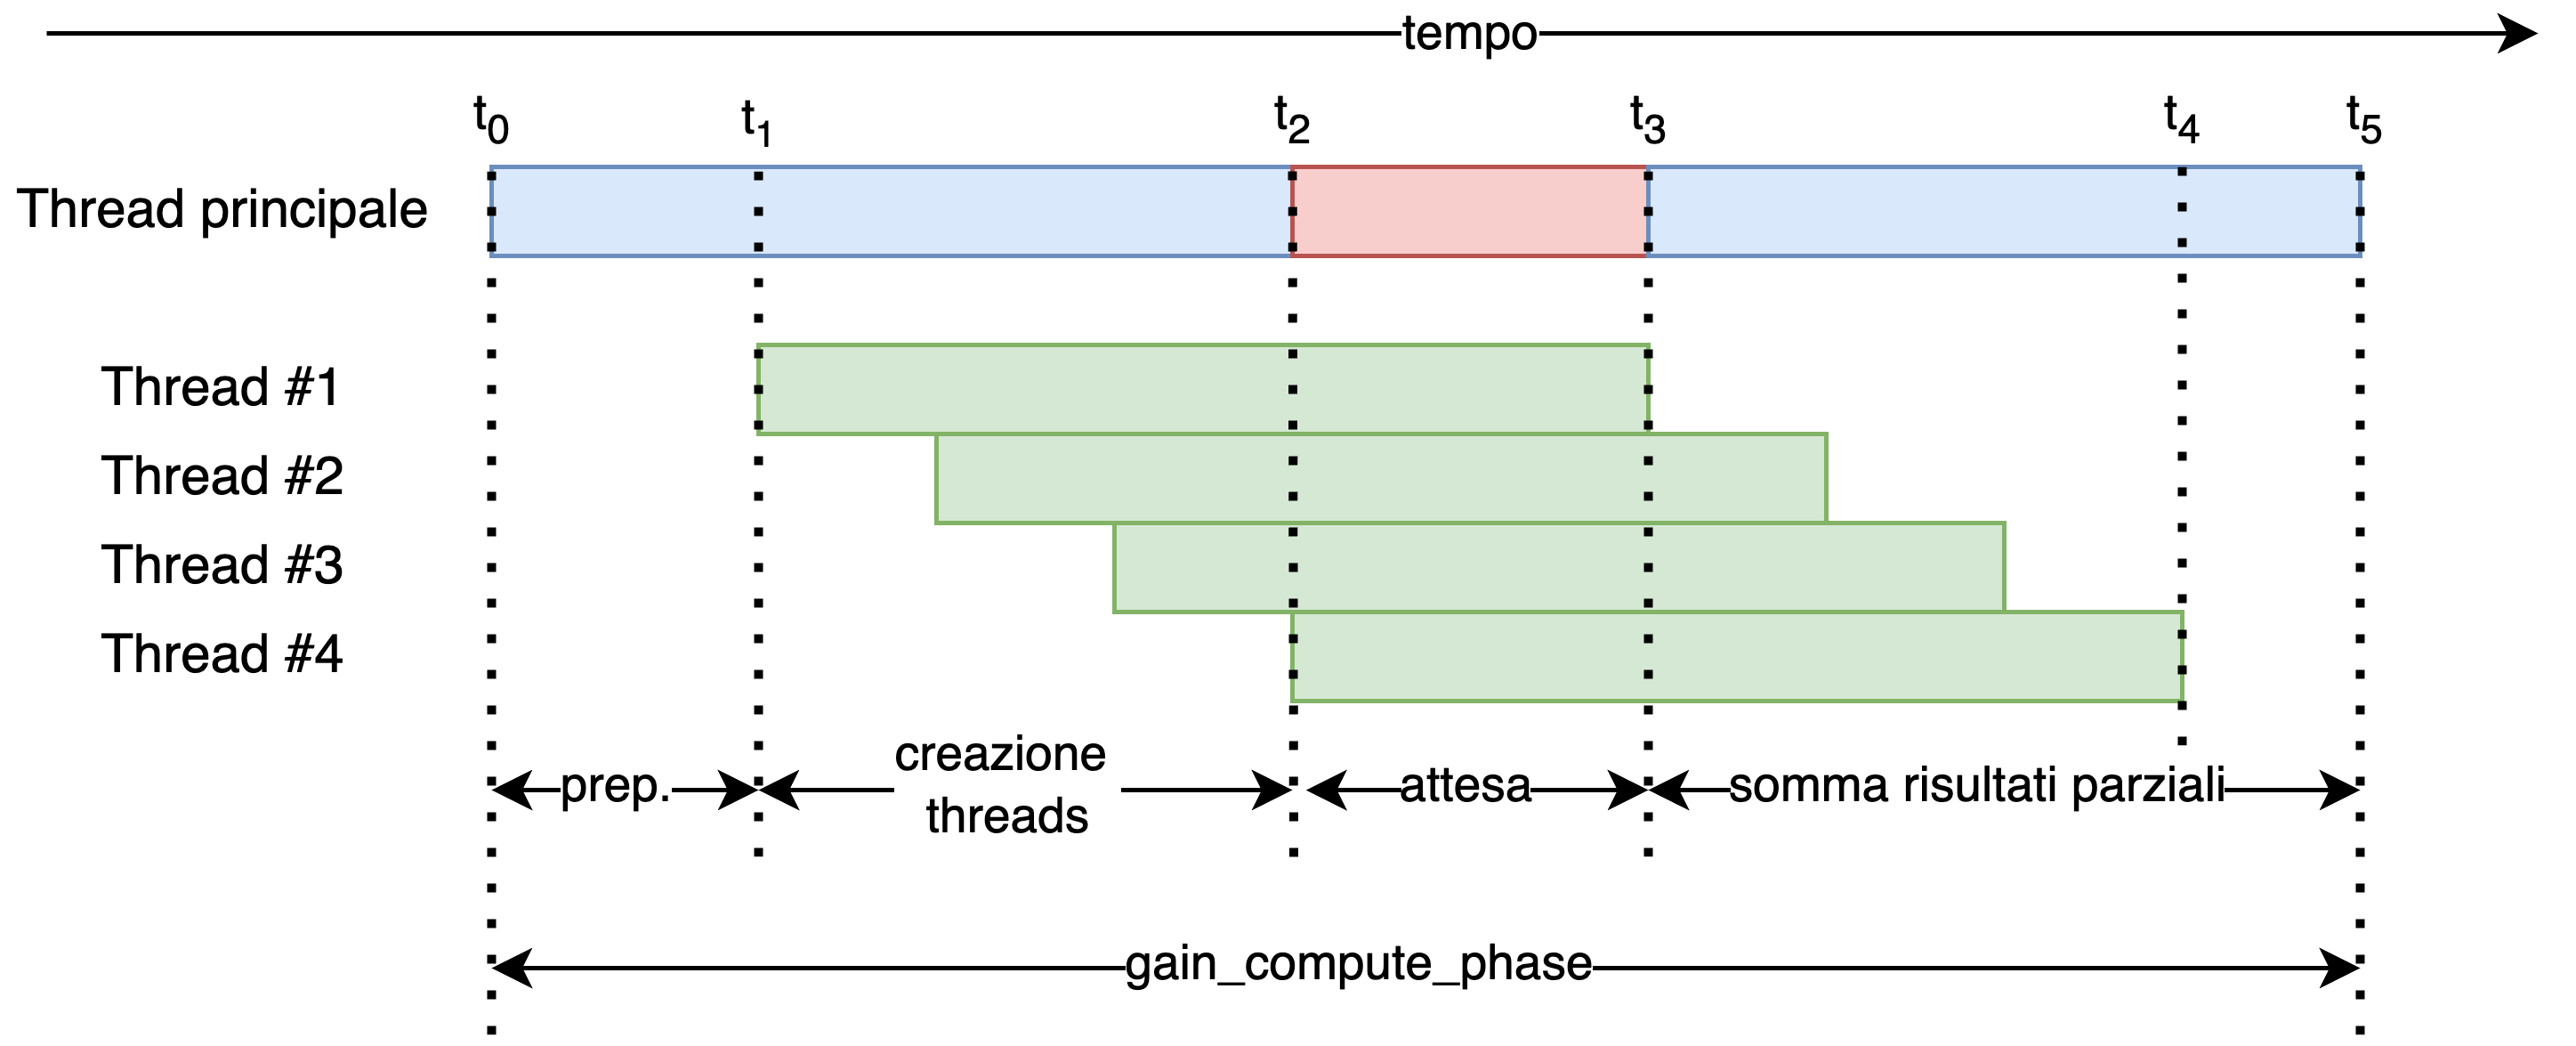
\includegraphics[width=\textwidth]{
    images/examples/gain_compute_phase-pipeline.png
  }
  \caption{Rappresentazione grafica della sequenza temporale delle operazioni
  eseguite da \texttt{gain\_compute\_phase}}
  \label{fig:gain-compute-phase-pipeline}
\end{figure}

\subsection{Parallelizzazione su GPU}
\label{subsec:cuda}

\lipsum[1]

\section{Discussione e Valutazione}
\label{ch:discussione}

\subsection{Vantaggi delle soluzioni implementate}
\label{subsec:vantaggi}

\lipsum[1]

\paragraph{Performance e tempo di esecuzione}
\label{para:performance}

\lipsum[1]

\paragraph{Supporto multi-piattaforma}
\label{para:supporto}

\lipsum[1]

\subsection{Svantaggi delle soluzioni implementate}
\label{sec:svantaggi}

\lipsum[1]

\paragraph{Leggibilità e manutenibilità del codice}
\label{para:leggibilita}

\lipsum[1]

\paragraph{Richiesta di hardware dedicato}
\label{para:hardware}

\lipsum[1]

\paragraph{Richiesta di conoscenze specifiche}
\label{para:conoscenze}

\lipsum[1]

\subsection{Limiti e sfide affrontate}
\label{subsec:limiti}

\lipsum[1]